\colorlet{mivertexcolor}{blue}
\colorlet{jivertexcolor}{red}
\colorlet{vertexcolor}{mivertexcolor!50}
\colorlet{bordercolor}{black!80}
\colorlet{linecolor}{gray}
% parameter corresponds to the used valuation function and can be addressed by #1
\tikzset{vertexbase/.style 2 args={semithick, shape=circle, inner sep=2pt, outer sep=0pt, draw=bordercolor},%
  vertex/.style 2 args={vertexbase={#1}{}, fill=vertexcolor!45},%
  mivertex/.style 2 args={vertexbase={#1}{}, fill=mivertexcolor!45},%
  jivertex/.style 2 args={vertexbase={#1}{}, fill=jivertexcolor!45},%
  divertex/.style 2 args={vertexbase={#1}{}, top color=mivertexcolor!45, bottom color=jivertexcolor!45},%
  conn/.style={-, thick, color=linecolor}%
}
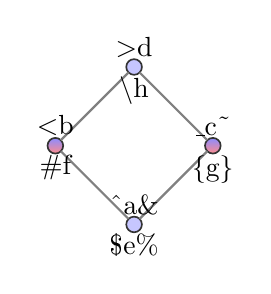
\begin{tikzpicture}
  \begin{scope} %for scaling and the like
    \begin{scope} %draw vertices
      \foreach \nodename/\nodetype/\param/\xpos/\ypos in {%
        0/vertex//0/0,
        1/divertex//-1/1,
        2/divertex//1/1,
        3/vertex//0/2
      } \node[\nodetype={\param}{}] (\nodename) at (\xpos, \ypos) {};
    \end{scope}
    \begin{scope} %draw connections
      \path (2) edge[conn] (3);
      \path (0) edge[conn] (2);
      \path (1) edge[conn] (3);
      \path (0) edge[conn] (1);
    \end{scope}
    \begin{scope} %add labels
      \foreach \nodename/\labelpos/\labelopts/\labelcontent in ,
        1/below//{\#f},
        2/below//{\{g\}},
        3/below//{\textbackslash h}
      } \coordinate[label={[\labelopts]\labelpos:{\labelcontent}}](c) at (\nodename);
    \end{scope}
  \end{scope}
\end{tikzpicture}
